\chapter[High Level Overview]{Chapter 3: High Level Overview}\label{chap:HL_overview}
%*******************************************%
\section{Summary}\label{sec:intro_HLovv}
This chapter offers a high-level overview of the project. The "Concept Investigation" section explores the methodology underpinning the project's core idea. The "Design Requirements" section outlines critical specifications and constraints guiding the design. The "Scalable Architecture" section examines the design's adaptability to varying scales and configurations. Lastly, the "Hypothesis \& Potential Drawbacks" section discusses assumptions and possible challenges encountered in the design process.
%*******************************************%
\section{Concept Investigation}\label{sec:consep}
%*******************************************%
The mainstream approach towards Battery Management Systems (BMS) for large battery banks in the industry has traditionally hinged on robust BMS controllers adept at managing long series cell strings. These systems are generally designed with a fixed cell management capacity, thereby lacking inherent scalability. The prevalent paradigm encapsulates a fixed number of cells within a module, each equipped with its dedicated BMS. These modules can then be arranged in series, with each BMS capable of inter-module communication, facilitating a level of scalability as depicted in the following diagram:

\begin{figure}[h!]
\centering
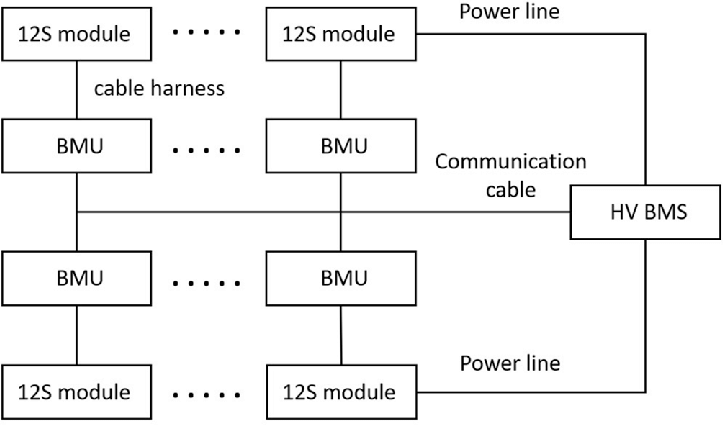
\includegraphics[width=0.4\textwidth]{Skripsie_LaTeXTemplate/Figures/HV_BANK_diaaa.png}
\caption{Conventional BMS approach for a high voltage battery bank\cite{generic}}
\label{fig:Conventional}
\end{figure}
\noindent
However, this conventional methodology manifests certain limitations upon scaling, primarily due to the introduction of inaccurate measurements and control constraints. The inaccuracies might stem from the cumulative error propagation and latency in communication as the number of series-connected modules escalates. Moreover, the fixed design poses a barrier to seamless scalability and flexibility in system expansion.\newline\newline
\noindent
To transcend these limitations and achieve enhanced accuracy in cell monitoring, a novel concept is proposed. Rather than modularizing a group of cells with a shared BMS, each cell is envisioned to be accompanied by its individual monitoring system. The core of this innovative design lies in stacking cells each endowed with its own monitoring system, thereby circumventing the scalability constraints imposed by traditional designs. The scalability in this scenario is principally governed by the communication bandwidth and line impedance between the monitoring systems.\newline\newline
\noindent
The proposed design envisages a miniature module atop each cell, housing monitoring components and a dedicated micro-controller, thereby rendering an individualized BMS for every cell. While the prototype is tailored for four cells, the intrinsic design flexibility enables scaling up to accommodate high voltage battery banks by merely augmenting the system with additional cells and modules.\newline\newline
\noindent
This modular BMS design essentially mirrors the architecture of a conventional BMS but miniaturizes it to fit atop each cell independently. Consequently, every cell in the series string is furnished with a parallel-connected monitoring module. Each of these modules, equipped with its micro-controller, is tasked with processing measurements and relaying the data to a central master device for either storage or further dissemination. The interconnection among all boards facilitates seamless communication, thereby fostering a comprehensive understanding of the battery pack's state across all modules. This collective insight empowers each module to evaluate the global state of the battery pack and fine-tune its respective cell’s variables accordingly. The following diagram elucidates the conceptual design of this novel BMS architecture:

\begin{figure}[h!]
\centering
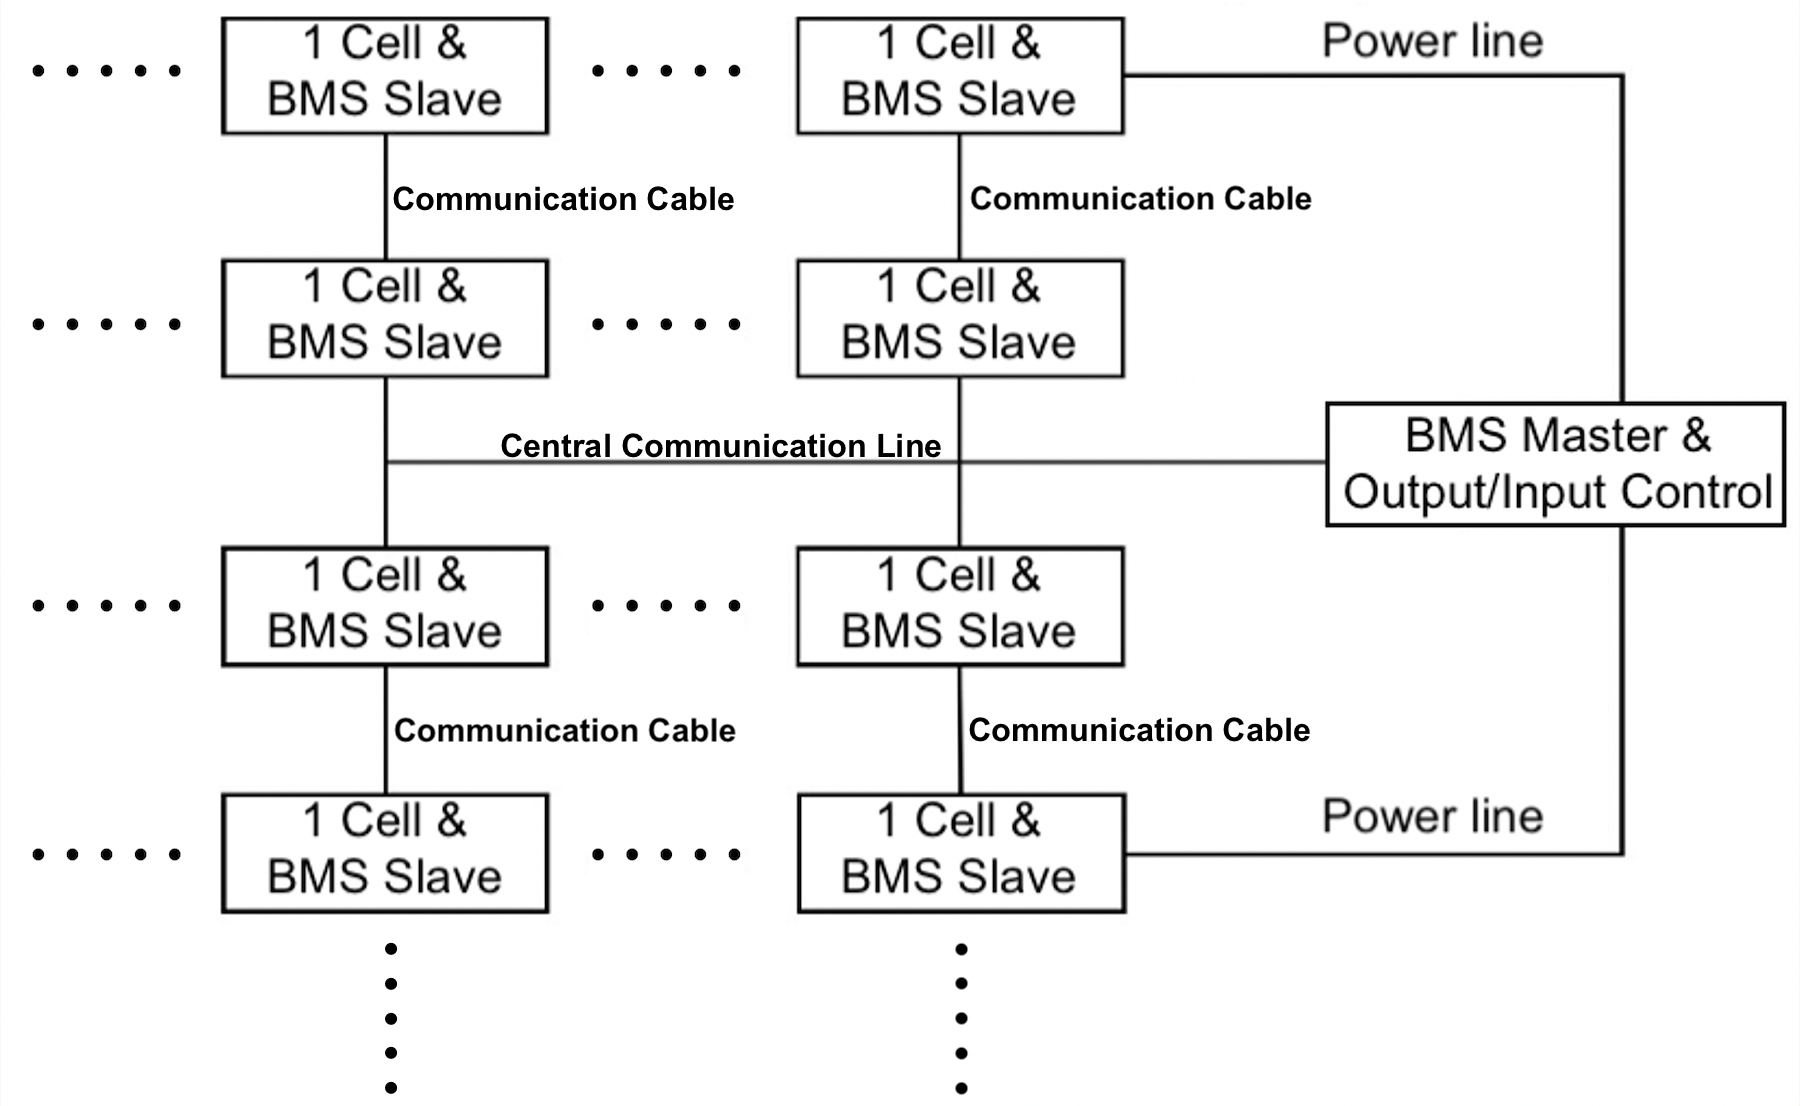
\includegraphics[width=0.5\textwidth]{Skripsie_LaTeXTemplate/Figures/NEW_HV_BANK_diaaa.png}
\caption{Concept Design for a modular BMS}
\label{fig:Conventional1}
\end{figure}
%*******************************************%
\section{Design Requirements}\label{sec:DesignReq}
%*******************************************%
The concept design investigated above will be developed in the hardware design of the system to meet requisites for the Battery Management System (BMS) aimed at ensuring modularity, scalability, and reliable performance.

\begin{itemize}
    \item \textbf{Modularity and Scalability}: The BMS is designed to independently monitor an extendable number of cells through dedicated subsystems for each cell. The initial prototype will monitor four cells, with scalability being a core attribute to accommodate a potentially indefinite number of cells.
    
    \item \textbf{Communication}: Serial communication via Universal Asynchronous Receiver/Transmitter (UART) protocol will be established among cell monitoring modules and between the modules and the master controller. Isolation in communication is required to handle different voltage levels across the string of cells.
    
    \item \textbf{Safety Features}: Essential safety features include cell temperature monitoring, cell voltage monitoring, cell balancing, string current monitoring, a reliable relay disconnect mechanism for anomaly detection, force reset functionality for non-responsive scenarios, and over-current protection facilitated through fuses.
    
    \item \textbf{Cell Monitoring}: Optimized for 105 Ah LFP cells, the design targets maintaining cell terminal voltage within 3.35V to 3V for operational longevity. Accurate voltage monitoring is required, with a preliminary accuracy of around ±0.05\%. Although cell temperature monitoring does not necessitate high accuracy, exceptional reliability is mandatory.
    
    \item \textbf{Cell Balancing}: Passive balancing will be employed, with each monitoring module hosting a dedicated dump load circuit targeting a balancing current of around 1A per cell, aligning with the good practice of 1\% of the cell's current capacity.
    
    \item \textbf{Power Supply}: Cell monitoring modules will be powered individually by the respective cells they are monitoring, with cell voltage boosted to a constant 5V for logic level optimization. The master controller will be powered from the series string of four cells through a buck supply delivering 5V.
    
    \item \textbf{Physical Constraints}: The monitoring modules' PCB dimensions are constrained to approximately 40mm x 40mm to fit between the cell terminals and edges of the cell.
    
    \item \textbf{Data Rate}: While there is no specific requirement for the data rate, a fairly fast rate is desired. The precise data rate will be determined during the serial communication design phase, and data integrity assurance is not a priority as the design will be used prototype-based.
\end{itemize}
%*******************************************%
\section{Scalable Architecture}\label{sec:scale_HLovv}
%*******************************************%
The proposed BMS architecture employs individual cell monitoring modules in parallel with each cell in a battery bank, addressing key scalability issues:

\begin{enumerate}
    \item \textbf{Wiring Complexity}: Utilizes four short wires per module for communication and cell terminal connections, minimizing wiring harness and failure risks.
    \item \textbf{Switching and Sizing}: Independent monitoring and dedicated balancing load per module ensure precise switching and optimal sizing.
    \item \textbf{Single-Cell Focus}: Individualized monitoring eliminates multicell complications, with inter-module communication ensuring coherent system understanding.
    \item \textbf{Scalable BMS Architecture Pathway}: The modular design inherently scales with battery bank expansion, promoting a seamless, scalable BMS architecture.
\end{enumerate}
\noindent
This architecture significantly mitigates conventional scalability challenges, warranting further research and development for efficient, scalable BMS solutions.
%*******************************************%
\section{Hypothesis \& Potential Drawbacks}\label{sec:drawbacks}
%*******************************************%
This project aims to advance high voltage battery management system (BMS) innovations by designing and evaluating a modular cell monitoring system. The goal is to explore a novel BMS architecture that could inspire future models and enhance the management of LFP cells at high voltages. Although the initial design iteration may not be ready for real-world application, it will provide a foundation for understanding the principles and configurations fundamental to a modular BMS for LFP batteries. The initial phase will focus on experimental design and analysis.\newline\newline
\noindent
The development will involve a comprehensive process of design and conceptualization to establish a foundational evaluation framework. Given the complex nature of electronic design, encountering unforeseen challenges is expected and listing all potential drawbacks would be impractical. The project's scope may expand due to its multidimensional nature, necessitating strict adherence to a research, design, develop, and evaluate cycle to maintain focus. The timeline is structured to permit only a single design iteration, provided there are no deviations from the planned path.\newline\newline
\noindent
Component availability and procurement delays are anticipated to affect the schedule, potentially compressing the time available for evaluation. Given the project's scale and timeframe, debugging and design reviews will likely proceed in parallel. Strategies to mitigate time delays include task overlapping, which aims to streamline the project's workflow and minimize disruptions.
%*******************************************%




\vfill
